\section{Closure with nearest particle statistics}

To circumvent the issue of diverging integral we introduce the \textit{nearest neighbor statistic} of \citet{zhang2021ensemble}. 
As the computation of the velocity disturbance of the droplets requires the knowledge of its center of mass velocity, we slightly modify the \textit{Nearest neighbor statistics} of \citet{zhang2021ensemble} to include a condition on the \textit{test} particle, regarding its center of mass velocity.
Therefore,  we introduce the \textit{Nearest neighbor velocity-included} distribution as, 
\begin{equation}
    P_\text{nst}^f[\textbf{x},\textbf{r},\textbf{w},t]
    = \frac{1}{\phi_f}\avg{
        \chi_f[\textbf{x},t]
        \sum_i^N 
        \delta(\textbf{x}_i[\FF,t]-\textbf{y})
        \delta(\textbf{u}_i[\FF,t]-\textbf{w})
        h_i[\textbf{x},\FF,t]
    },
\end{equation}
where,
\begin{align}
    \label{eq:h_i_def}
    h_i[\textbf{x},\FF,t]
    = \frac{1}{N[\textbf{x},t,\FF]}
    \prod_j H(|\textbf{x}_j[\FF,t] - \textbf{x}| - |\textbf{x}_i[\FF,t] - \textbf{x}|)\\
    \label{eq:N_def}
    N[\textbf{x},t,\FF]
    = \sum_i\prod_jH(|\textbf{x}_j[\FF,t] - \textbf{x}| - |\textbf{x}_i[\FF,t] - \textbf{x}|).
\end{align}
It must be understood from this definition that $h_i=1$ if and only if the particle $i$ is the nearest neighbor to the point $\textbf{x}$. 
From this definition, $P_\text{nst}^f$ is the probability of finding the nearest neighbor of the point \textbf{x} at \textbf{y}, with a center of mass velocity, \textbf{w}, knowing that the continuous phase is present at \textbf{x} and at time $t$. 

By noticing that, 
\begin{equation}
    \int_{\mathbb{R}^6}
    \sum_i^N 
    \delta(\textbf{x}_i[\FF,t]-\textbf{y})
    \delta(\textbf{u}_i[\FF,t]-\textbf{w})
    h_i[\textbf{x},\FF,t]
    d\textbf{r}
    d\textbf{w} 
    =1,
\end{equation}
we arrive at the same conclusion as \citet{zhang2021ensemble} and write, 
\begin{equation}
    \avg{f_f^0\chi_f}
    = 
    \int_{\mathbb{R}^6}
    (f_f^\text{nst}P_\text{nst}^f\phi_f)[\textbf{x},\textbf{r},\textbf{w},t]
    d\textbf{r}
    d\textbf{w}
    \label{eq:ensemble_avg_to_nst}
\end{equation} 
where $f_f^0[\textbf{x},\FF,t]$ is an arbitrary property pertaining to the continuous phase, and $f_f^\text{nst}[\textbf{x},t|\textbf{w},\textbf{y}]$ its nearest neighbor conditional average, namely, 
\begin{equation}
    f_f^\text{nst}[\textbf{x},t|\textbf{w},\textbf{y}]
    =\frac{1}{(P_\text{nst}^f\phi_f) [\textbf{x},\textbf{r},\textbf{w},t]}
    \avg{
        (f_f^0
        \chi_f)[\textbf{x},t]
        \sum_i^N 
        \delta(\textbf{x}_i[\FF,t]-\textbf{y})
        \delta(\textbf{u}_i[\FF,t]-\textbf{w})
        h_i[\textbf{x},\FF,t]
    }.
    \label{eq:def_f_nst}
\end{equation}
Note that the only difference between these definitions and, Equation (2.6) to (2.8) of \citet{zhang2021ensemble}, is the inclusion of $\delta(\textbf{u}_i - \textbf{w})$ in our formulas. 
Anyhow, \ref{eq:ensemble_avg_to_nst} permitted us to express any ensemble-averaged quantities in terms of \textit{Nearest neighbor conditioned} quantities. 
Therefore, this formula is similar to \ref{eq:batchlor_avg}, in that it provides a link between ensemble and conditional average, but derived without any assumption, and as a result no errors. 

In the following, we introduce the shorthand, 
\begin{equation*}
    \delta_\text{nst}
    =
    % \chi_f
    \sum_i^N 
    \delta(\textbf{x}_i[\FF,t]-\textbf{y})
    \delta(\textbf{u}_i[\FF,t]-\textbf{w})
    h_i[\textbf{x},\FF,t],
    \label{eq:def_delta_nst}
\end{equation*}
so that the \textit{nearest neighbor  conditional  average} can simply be written, $f_f^\text{nst} P_\text{nst}^f \phi_f = \avg{\chi_f f_f^0 \delta_\text{nst}}$.

\subsection{Formulation of the Reynolds stress tensor}

Now, let us apply \ref{eq:ensemble_avg_to_nst} with $f_f^0 = \textbf{u}_f'\textbf{u}_f'$, it yields,
\begin{equation}
    \avg{\chi_f \textbf{u}_f'\textbf{u}_f'}
    = 
    \phi_f
    \int_{\mathbb{R}^6}
    \textbf{v}_f^\text{nst}
    \textbf{v}_f^\text{nst}
    P_\text{nst}^f
    d\textbf{y}
    d\textbf{w}
    + 
    \int_{\mathbb{R}^6}
    \avg{
        \chi_f
        \textbf{u}_f''
        \textbf{u}_f''
        % \sum_i 
        % \delta(\textbf{x}+\textbf{y}-\textbf{x}_i)
        % \delta(\textbf{w}-\textbf{u}_i)
        % h_i
        \delta_\text{nst}
    }
    d\textbf{y}
    d\textbf{w}.
    \label{eq:relation_ensemble_nst}
\end{equation}
Where we have defined 
the fluctuation of the local value of the fluid phase velocity around the nearest neighbor conditional average velocity, $\textbf{u}_f'' = \textbf{u}_f^0 - \textbf{u}_f^\text{nst}$, and the fluctuation of the nearest neighbor conditional average, velocity around the ensemble average velocity, that is $\textbf{v}_f^\text{nst} = \textbf{u}_f^\text{nst} - \textbf{u}_f$. 
In the first term on the right-hand side of \ref{eq:relation_ensemble_nst}, it is important to note that $\phi_f$ depends only on $\textbf{x}$ and $t$. 
This allows us to treat $\phi_f$ as a constant with respect to the variables of integration, making it possible to factor out $\phi_f$.
According to \ref{eq:relation_ensemble_nst}, 
we state that we can separate the \textit{Reynolds stress} tensor into two distinct contributions :  (1) The agitation generated by the \textit{nearest neighbor conditionally averaged} wakes, denoted by $\textbf{v}_f^\text{nst}$, and (2) all other sources of fluctuations, such as those arising from particle interactions and single-phase turbulence, represented by $\textbf{u}_f''$. 
Note that, this decomposition is similar to \ref{eq:classic_avg,eq:batchlor_avg}, the only difference is the presence of the \textit{nearest neighbor conditionally averaged} fields instead of the classic \textit{single-particle conditionally averaged} fields. 

To give a better physical explanation of what is $\textbf{u}_f^\text{nst}$ we display on \ref{fig:unst} an instantaneous representation of its meaning. 
\begin{figure}[h!]
    \centering
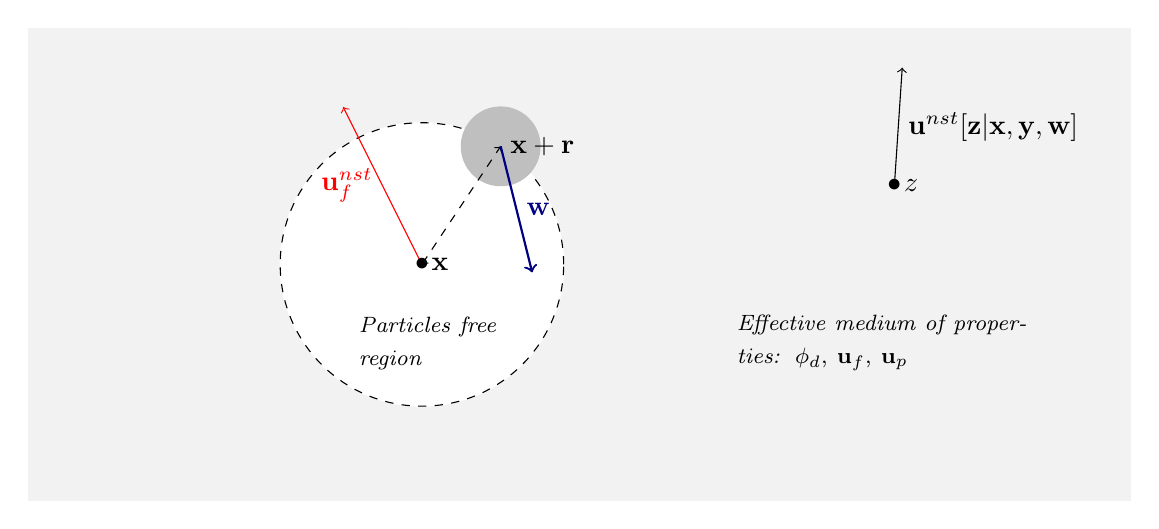
\begin{tikzpicture}
    \filldraw[gray!10](-5,-3) rectangle(9,3);
    \filldraw[white](0,0) circle (1.8);
    \filldraw[ gray!10!white](+2.6,0.5)circle (0.5);
    \filldraw[ gray!10!white](-1.5,2.2)circle (0.5);
    \draw[dashed](0:1.8) arc (0:360:1.8);
    % \filldraw[ gray!50!white](0,0) circle (0.5);
    \filldraw[ gray!50!white](1,1.5)circle (0.5);
    \filldraw[ gray!10!white](-0.2,2.5)circle (0.5);
    \draw[->,red](0,0)--++(-1,2)node[midway,left]{$\textbf{u}_f^\text{nst}$};
    \draw(0,0)node{$\bullet$}node[right]{$\textbf{x}$};
    \draw[dashed,<->](0,0)--(1,1.5)node[right]{$\textbf{x}+\textbf{r}$};
    \draw[->,blue!50!black,thick](1,1.5)--++(0.4,-1.6)node[midway,right]{$\textbf{w}$};
    % \draw[dashed](-0.2,3.5);
    \node[text width=2cm] (title) at (0.2,-1) {\footnotesize\textit{Particles free region}};
    % \node[ultra thick] (title) at (-0.5,-1.5) {(\textit{Case 1})};
    \node[text width=4cm] (title) at (6,-1) {\footnotesize\textit{Effective medium of properties:} $\phi_d$, $\textbf{u}_f$, $\textbf{u}_p$};
    \draw[->] (6,1)node{$\bullet$}node[right]{$z$}--++(0.1,1.5)node[right,midway]{$\textbf{u}^\text{nst}[\textbf{z}|\textbf{x},\textbf{y},\textbf{w}]$};
\end{tikzpicture} 
\caption{Representation of the \textit{nearest neighbor conditionally averaged} velocity fields $\textbf{u}_\text{nst}^f[\textbf{x},\textbf{w},\textbf{r},t]$.
Figure adapted from (Figure 2) of \citet{zhang2021ensemble}}
\label{fig:unst}
\end{figure}
According to \ref{eq:def_f_nst} and \ref{fig:unst} $\textbf{u}_f^\text{nst}[\textbf{x},\textbf{r},\textbf{w}]$ is the averaged value of $\textbf{u}_f^0$, evaluated at \textbf{x}, on all configuration where the nearest droplet is present at $\textbf{y} = \textbf{x} + \textbf{r}$ with velocity $\textbf{w}$. 
Consequently, the region delimited by the sphere, centered at \textbf{x} of radius $|\textbf{y} - \textbf{x}|$ must be empty of particles center of mass since the closest neighboring droplet is at \textbf{y} \citep{zhang2021ensemble}. 
The region outside this particle-free region corresponds therefore to an effective medium where both the particle and the fluid phase are averaged conditionally on the configuration represented by $\chi_f\delta_\text{nst}$. 
This deeper physical understanding will prove valuable in the subsequent section.  
We argue however that the particle-free zone as defined by \ref{fig:unst} is incomplete. 
Indeed, inside the spherical shell of radius $2a$ centered at $\textbf{y}$ no center of mass of droplets can be present due to the impenetrability of the droplets. 
However, we neglect this term for now. 


In summary, we reformulated the ensemble-averaged \textit{Reynolds stress} tensor using a well-normed conditional average \eqref{eq:def_f_nst} based on the nearest particle's position and velocity. 
However, in this phase-space, $\textbf{v}_f^\text{nst}$ is not merely the velocity field around a particle but rather the velocity field averaged over a specific scenario, as illustrated in \ref{fig:unst}. 

\subsection{Equations for the nearest neighbor averaged velocity fields. }

To compute the sedimentation velocity in non-dilute suspensions of hard spheres, \citet[Appendix B]{zhang2021ensemble} derived the field $\textbf{u}_f^\text{nst}$ using the \textit{nearest neighbor conditionally averaged} Navier-Stokes equations. 
% As the derivation lacks detailed proof, particularly regarding the steps leading to Equation (B 1) of \citet{zhang2021ensemble}, 
We present in this section a systematic methodology for deriving these conditionally averaged equations. 

Inspired by the classic conditional average methodology of \citet{hinch1977averaged}, we propose that the \textit{nearest neighbor conditionally averaged} velocity fields, i.e., $\textbf{v}_f^\text{nst}$, can be obtained by conditionally averaging the local-scale mass and momentum equations, and then solving the resulting equations for $\textbf{v}_f^\text{nst}$. 
Thus, we first recall the local mass and momentum equations, 
\begin{align}
    \pddt (\rho_f\chi_f) +  \pddx \cdot (\rho_f\chi_f\textbf{u}^0_f) &= 0 
    \label{eq:local_equations_mass}
    \\
    \pddt (\rho_f\chi_f\textbf{u}^0_f)
    + \pddx\cdot (\rho_f\chi_f\textbf{u}^0_f\textbf{u}^0_f - \chi_f\bm\sigma^0_f)
    &= 
    - \delta_\Gamma \bm\sigma_f^0 \cdot \textbf{n}_d. 
    + \chi_f \rho_f \textbf{g}
    \label{eq:local_equations_mom}
\end{align}
Note that, at this stage, the inertial terms cannot be neglected since the momentum equation is not yet expressed in the reference frame of the droplet at \textbf{y}. 
Then, note that we can obtain $\textbf{v}_f^\text{nst}$ from $\textbf{u}_f^0$ directly through the averaging procedure: 
\begin{equation}
    \textbf{v}_f^\text{nst} P_\text{nst}^f
    % = 
    % \textbf{u}_f^\text{nst} P_\text{nst}^f
    % - \textbf{u}_f P_\text{nst}^f
    = 
    \avg{\delta_\text{nst} \chi_f \textbf{u}_f^0}
    - \textbf{u}_f P_\text{nst}^f
\end{equation}
We deduce that to obtain an equation for $\textbf{u}_f^\text{nst}$ we must multiply, \ref{eq:local_equations_mass} and \ref{eq:local_equations_mom} that are evaluated at \textbf{x}, by $\delta_\text{nst}$ and average over all configurations. 
This introduces the need for a conservation equation for the distribution $\delta_\text{nst}$ since this distribution does not commute with the time and space derivative. 

\subsubsection{Conditionally mass transport equation}

By taking the partial time derivative of each distribution present in \ref{eq:def_delta_nst} independently, we obtain the conservation equations, 
\begin{align}
    \label{eq:dt_delta_x}
    \pddt \delta(\textbf{x}_i  - \textbf{y})
    +\textbf{u}_i  
    \cdot \pddy \delta(\textbf{x}_i  - \textbf{y})
    = 0\\
    \pddt \delta(\textbf{u}_i -\textbf{w})
    +\textbf{a}_i \cdot  \pddw   \delta(\textbf{u}_i  - \textbf{w})
    = 0\\
    \pddt \chi_f 
    + \textbf{u}_\Gamma^0 
    \cdot \pddx \chi_f = 0 \\
    \pddx \chi_f = - \delta_\Gamma \textbf{n}_f,
    \label{eq:chi_f_dt}
\end{align}
where we recall that $\textbf{u}_\Gamma^0$ is the velocity of the droplets interfaces, and $\textbf{n}_f$ is the normal pointing inward the droplets surfaces. 
Additionally, The vector $\textbf{a}_i = \ddt \textbf{u}_i$ corresponds to the center of mass acceleration of the particle $i$. 
From the conservation laws given by \ref{eq:dt_delta_x} to \ref{eq:chi_f_dt}, we deduce that, 
\begin{align}
    \pddt \delta_\text{nst}
    + \pddy \cdot (\textbf{w} \delta_\text{nst})
    + \pddw \cdot (\textbf{a}_i  \delta_\text{nst})
    = 
    \sum_i \delta(\textbf{x}_i -\textbf{y}) \delta(\textbf{u}_i - \textbf{w}) \pddt h_i
\end{align}
% and, 
% \begin{align*}
%     \pddt (\chi_f \delta_\text{nst})
%     + \pddy \cdot (\textbf{w} \chi_f \delta_\text{nst})
%     + \pddw \cdot (\textbf{a}_i  \chi_f \delta_\text{nst})
%     = 
%     \chi_f \delta(\textbf{x}_i -\textbf{y}) \delta(\textbf{u}_i - \textbf{w}) \pddt h_i
%     + \delta_\Gamma \delta_\text{nst} \textbf{u}_\Gamma\cdot \textbf{n}_f
% \end{align*}
Additionally, it can be shown that,
\begin{align}
    \pddt  h_i[\textbf{x},t,\FF]
    = 
    h_i
    \sum_k 
    \delta(r_k - r_i)
    (\textbf{u}_k  \cdot \hat{\textbf{r}}_k - \textbf{u}_i  \cdot \hat{\textbf{r}}_i)\\
    \pddx  h_i[\textbf{x},t,\FF]
    = 
    h_i
    \sum_k 
    \delta(r_k - r_i)
    ( \hat{\textbf{r}}_k -  \hat{\textbf{r}}_i),
    \label{eq:dt_h_i}
\end{align}
where $\textbf{u}_k$ and $\textbf{u}_i$  are the center of mass velocity of the particle $k$ and $i$, respectively.
Note that the second expression agrees with \citet[Appendix A]{zhang2021ensemble}. 
We also introduced the notation $r_i$ and $r_k$ which represents the radial distance from the particle $i$ to the point $\textbf{x}$ namely, $r_i = |\textbf{x}_i - \textbf{x}|$.  
Considering \ref{eq:dt_h_i}  yields an expression for the transport equation of $\delta_\text{nst}$ namely,
\begin{equation}
    \pddt \delta_\text{nst}
    + \pddy \cdot (\textbf{w} \delta_\text{nst})
    + \pddw \cdot (\textbf{a}_i  \delta_\text{nst})
    = 
    % \sum_i
    % \delta(\textbf{x}_i -\textbf{y}) 
    % \delta(\textbf{u}_i - \textbf{w}) 
    \delta_\text{nst}
    % h_i
    \sum_k 
    \delta(r_k - r_i)
    (\textbf{u}_k  \cdot \hat{\textbf{r}}_k - \textbf{u}_i  \cdot \hat{\textbf{r}}_i). 
    \label{eq:dt_delta_nst_start}
\end{equation}
As demonstrated in \citet{zhang2023evolution}, the right-hand side term of \ref{eq:dt_delta_nst_start} represents the source terms due to the permutation of nearest neighbor to the point \textbf{x}. 
For reasons that will become clear later on, we add the term $\textbf{u}_f^0\cdot \pddx \delta_\text{nst}$ on each side of \ref{eq:dt_delta_nst_start}, which gives,
\begin{equation}
    \pddt \delta_\text{nst}
    + \textbf{u}_f^0\cdot \pddx \delta_\text{nst}
    + \textbf{w}   \cdot \pddy \delta_\text{nst}
    + \textbf{a}_i \cdot \pddw   \delta_\text{nst}
    = 
    % \sum_i
    % \delta(\textbf{x}_i -\textbf{y}) 
    % \delta(\textbf{u}_i - \textbf{w}) 
    \delta_\text{nst}
    % h_i
    \sum_k 
    \delta(r_k - r_i)
    [(\textbf{u}_k - \textbf{u}_f^0) \cdot \hat{\textbf{r}}_k - (\textbf{u}_i  - \textbf{u}_f^0)\cdot \hat{\textbf{r}}_i]. 
    \label{eq:dt_delta_nst}
\end{equation}
Where on the right-hand side of \ref{eq:dt_delta_nst} we have reformulated the term $\textbf{u}_f^0\cdot \pddx \delta_\text{nst}$, using \ref{eq:dt_h_i}. 

To derive an equation for $\phi_f P_\text{nst}^f = \avg{\chi_f \delta_\text{nst}}$ we multiply \ref{eq:dt_delta_nst} by $\chi_f$, and use \ref{eq:chi_f_dt}, namely
\begin{multline}
    \pddt (\chi_f\delta_\text{nst})
    +  \pddx \cdot (\textbf{u}_f^0 \chi_f\delta_\text{nst})
    +  \pddy \cdot (\textbf{w}    \chi_f\delta_\text{nst})
    +  \pddw \cdot   (\textbf{a}_i  \chi_f\delta_\text{nst})\\
    = 
    % \sum_i
    % \delta(\textbf{x}_i -\textbf{y}) 
    % \delta(\textbf{u}_i - \textbf{w}) 
    (\chi_f\delta_\text{nst})
    % h_i
    \sum_k 
    \delta(r_k - r_i)
    [(\textbf{u}_k - \textbf{u}_f^0) \cdot \hat{\textbf{r}}_k - (\textbf{u}_i  - \textbf{u}_f^0)\cdot \hat{\textbf{r}}_i],
    \label{eq:dt_delta_nst_chi}
\end{multline}
which upon averaging gives directly,
\begin{multline}
    \pddt (\phi_fP_\text{nst}^f)
    + 
    \pddx \cdot (
        \phi_f 
        P_\text{nst}^f
        \textbf{u}_f^\text{nst}
    )
    + \pddy \cdot (
        \phi_f
        P_\text{nst}^f
        \textbf{w} 
    )
    +
    \pddw \cdot (  
        \phi_f 
        P_\text{nst}^f
        \textbf{a}_p^\text{nst} 
    )
    = \\
    + \avg{
    %  \chi_f \textbf{u}_\Gamma \cdot \pddx \delta_\text{nst}
     \chi_f \delta_\text{nst}
    \sum_k 
    \delta(r_k - r_i)
    [(\textbf{u}_k - \textbf{u}_\Gamma^0) \cdot \hat{\textbf{r}}_k - (\textbf{u}_i- \textbf{u}_\Gamma^0)  \cdot \hat{\textbf{r}}_i]}.
    \label{eq:dt_P_nst_chi}
\end{multline}
% where we have noted that $\textbf{u}_\Gamma^0 = \textbf{u}_f^0$ in the absence of mass transfer. 
In this relation, the left-hand side terms represent the advection of $\phi_f P_\text{nst}^f$ along the phase space variables ($t$, $\textbf{x}$, $\textbf{y}$ and $\textbf{w}$).
The source term on the right-hand side of \ref{eq:dt_P_nst_chi} accounts for the changes in nearest neighbor distribution due to the permutation of the nearest neighbor at the local scale. 
Note the similarities of the right-hand side source term of \ref{eq:dt_P_nst_chi} with (A10) of \citet{zhang2023evolution}, which derived a transport equation for $P_\text{nst}$, which is defined as the probability density of the nearest pairs of particles as it is described in \ref{chap:microstructure}. 
We remark that the source terms of (A10) \citet{zhang2023evolution} and \ref{eq:dt_P_nst_chi} yield the same form.
Still in \ref{eq:dt_P_nst_chi} the velocity $\textbf{u}_i$ and $\textbf{u}_k$ are evaluated with respect to the local velocity of the fluid $\textbf{u}_f^0$, while in \citet{zhang2023evolution} it is evaluated relative to the velocity of the particles centered at \textbf{x}. 


\ref{eq:dt_P_nst_chi} can also be written in ``conservative'' form using the conserving law, 
\begin{equation}
    \pddt \phi_f 
    + \div(
        \phi_f
        \textbf{u}_f 
        ) 
    = 0, 
\end{equation}
which gives, 
\begin{multline}
    \pddt P_\text{nst}^f
    + 
    \pddx \cdot (
        P_\text{nst}^f
        \textbf{u}_f^\text{nst}
    )
    + \pddy \cdot (
        P_\text{nst}^f
        \textbf{w}
    )
    +
    \pddw \cdot (  
        P_\text{nst}^f
        \textbf{a}_p^\text{nst} 
    )
    = \\
    + \frac{1}{\phi_f}\avg{
    %  \chi_f \textbf{u}_\Gamma \cdot \pddx \delta_\text{nst}
     \chi_f \delta_\text{nst}
    \sum_k 
    \delta(r_k - r_i)
    [(\textbf{u}_k - \textbf{u}_\Gamma^0) \cdot \hat{\textbf{r}}_k - (\textbf{u}_i- \textbf{u}_\Gamma^0)  \cdot \hat{\textbf{r}}_i]}.
    \label{eq:dt_Pc_nst_chi}
\end{multline}
this equation corresponds to the \textit{nearest neighbor conditional averaged} conservation equation for the continuous phase.
As the continuous phase density $\rho_f$ is constant, \ref{eq:dt_Pc_nst_chi} also corresponds to the  \textit{nearest neighbor conditional averaged} mass conservation equation.  

\subsubsection{First form of the conditional averaged momentum equation}
Now that the transport equation for $\delta_\text{nst}$ and $P_\text{nst}^f$ are properly derived we can derive the \textit{nearest neighbor conditionally averaged} momentum equation. 
Multiplying \ref{eq:local_equations_mom} by $\delta_\text{nst}$, and making use of \ref{eq:dt_delta_nst} and averaging overall configurations yields, 
\begin{multline}
    \pddt (\rho_f\phi_f P_\text{nst} \textbf{u}^\text{nst}_f)
    + \pddx\cdot (
        \rho_f\phi_fP_\text{nst}^f \textbf{u}^\text{nst}_f\textbf{u}^\text{nst}_f 
        +\bm\sigma_\text{nst}^\text{eq})
    + \pddy\cdot (\phi_fP_\text{nst}^f \textbf{w}\textbf{u}_f^\text{nst} )
    + \pddw\cdot (\phi_fP_\text{nst}^f \textbf{a}_p^\text{nst} \textbf{u}_f^\text{nst} )\\
    = 
    \phi_fP_\text{nst}^f  \rho_f \textbf{g}
    - \avg{\delta_\text{nst}\delta_\Gamma \bm\sigma_f \cdot \textbf{n}_d} 
    % - \avg{\chi_f \bm\sigma_f^0 \cdot \grad\delta_\text{nst}}
    +\avg{
        \delta_\text{nst}
        \chi_f \bm\sigma_f^0 \cdot
        \sum_k 
        \delta(r_k - r_i)
        [\hat{\textbf{r}}_k - \hat{\textbf{r}}_i]}\\
    +\avg{
        %  \chi_f \textbf{u}_\Gamma \cdot \pddx \delta_\text{nst}
         \textbf{u}_f^0\chi_f \delta_\text{nst}
        \sum_k 
        \delta(r_k - r_i)
        [(\textbf{u}_k - \textbf{u}_f^0) \cdot \hat{\textbf{r}}_k - (\textbf{u}_i- \textbf{u}_f^0)  \cdot \hat{\textbf{r}}_i]},
    \label{eq:momentum_avg_nst}
\end{multline}
with the effective stress $\bm\sigma_\text{nst}^\text{eq}$ defined as, 
\begin{equation}
    \bm\sigma_\text{nst}^\text{eq}=
    \avg{\rho_f\chi_f\delta_\text{nst} \textbf{u}''_f\textbf{u}''_f} 
    - P_\text{nst}^f \avg{\rho_f\chi_f\textbf{u}'_f\textbf{u}'_f} 
    - \phi_f P_\text{nst}^f \bm\sigma^\text{nst}_f. 
\end{equation}
The terms on the left-hand side of \ref{eq:momentum_avg_nst} represent the advection of the \textit{nearest neighbor conditional average} momentum along the phase space coordinate, plus the contribution of the \textit{nearest neighbor conditional average} viscous stresses $\bm\sigma^\text{nst}_f$
The first term on right-hand side of \ref{eq:momentum_avg_nst} corresponds to the momentum exchange between phases, but conditionally averaged. 
Specifically, $\avg{\delta_\text{nst}\delta_\Gamma \bm\sigma_f \cdot \textbf{n}_d} $ represents the exchange of momentum at \textbf{x}, conditioned on the presence of the interface at \textbf{x} with the nearest neighbor to the point \textbf{x} located at \textbf{y} with velocity \textbf{w}.
The second and third terms are the additional contribution of the convective and non-convective fluxes due to the birth or death of nearest neighbors. 

In this form \ref{eq:momentum_avg_nst} is hardly solvable. 
While, the boundary condition at the surface of the particle (centered at \textbf{y}) for the velocity $\textbf{u}_f^\text{nst}[\textbf{y}+a \textbf{n}, \textbf{y},\textbf{w}]$ is well-defined, there is a lack of boundary conditions infinitely far from the particle. 
Absolutely, since the velocity field $\textbf{u}_f^\text{nst}$ is conditioned on the velocity of the droplet, we can be certain that $\textbf{u}_f^\text{nst}\cdot \textbf{n} = \textbf{w}\cdot \textbf{n}$ for the points lying on the droplet surface. 
However, $\lim_{|\textbf{x}- \textbf{y}|\to \infty} \textbf{u}^\text{nst}_f$ is undefined, since in the same limits $P_\text{nst}^f = 0$.
In other words, infinitely far from the particle's center of mass, the velocity field $\textbf{u}^\text{nst}_f$ has no physical meaning, as the probability of finding the nearest neighbor to a point in the fluid at such a distance is zero.
This, lack of boundary condition at infinity makes, \ref{eq:momentum_avg_nst} unsolvable regardless of the possible assumption that could be made.

\subsubsection{Second form of the conditional averaged equations}

To settle this issue we follow \citet[Appendix B]{zhang2021ensemble} and propose to solve for an auxiliary but equivalent problem.
Indeed, as $\textbf{u}_f^\text{nst}$ lacks a boundary condition at infinity, we choose instead to solve for the field $\textbf{u}^\text{nst}$ which is defined as,  
\begin{equation*}
    P_\text{nst-f}[\textbf{y},\textbf{w},\textbf{x},t]\textbf{u}^\text{nst}[\textbf{z},t|\textbf{x},\textbf{y},\textbf{w}]
    = \avg{\delta_\text{nst-f}  \textbf{u}^0[\textbf{z},\FF,t]}
    \label{eq:def_u_z}
\end{equation*}
where, $\delta_\text{nst-f} = \chi_f[\textbf{x},t,\FF]\delta_\text{nst}[\textbf{y},\textbf{w}, \FF,t]$. 
We recall that $\textbf{u}^0 = \chi_f\textbf{u}_f^0 + \chi_d \textbf{u}_d^0$ is the local bulk velocity of the mixture. 
Additionally, $P_\text{nst-f}$ is defined as,
\begin{equation}
    P_\text{nst-f}[\textbf{x},\textbf{y},\textbf{w},t] = \phi_f[\textbf{x},t]P_\text{nst}^f[\textbf{y},\textbf{w},t|\textbf{x}] = \avg{\delta_\text{nst-f}}. 
\end{equation}
Note that we included the subscript $f$ in $P_\text{nst-f}$ to indicate that the probability distribution $\phi_f$ is not a condition but is rather part of the distribution $P_\text{nst-f}$.
Thus, $\textbf{u}^\text{nst}$ is the \textit{nearest neighbor conditionally averaged} bulk velocity field evaluated at $\textbf{z}$, knowing the fluid phase is present at $\textbf{x}$ with the nearest neighbor to \textbf{x} being located in \textbf{y} with center of mass velocity \textbf{w}. 
A graphical representation of $\textbf{u}^\text{nst}$ is given in \ref{fig:unst}.
With that definition, we have the following boundary condition far from the particle-free region, 
\begin{equation}
    \lim_{|\textbf{z} - \textbf{y}|\to \infty}
    \textbf{u}^\text{nst}[\textbf{z},t|\textbf{x},\textbf{y},\textbf{w}]
    = \textbf{u}[\textbf{z},t]. 
    % \lim_{|\textbf{z} - \textbf{y}|\to \infty}
    % \phi^\text{nst}[\textbf{z},t|\textbf{x},\textbf{y},\textbf{w}]
    % = \phi[\textbf{z},t],
    \label{eq:boundary}
\end{equation}
We recall that $\textbf{u} = \avg{\chi_f\textbf{u}_f^0 + \chi_d \textbf{u}_d^0}$. 
\ref{eq:boundary} indicates that, far from the particle-free region, the particle located at \textbf{y} has no influence on the averaged quantities.
Additionally, note that, $\textbf{u}^\text{nst}$ is related to $\textbf{u}_f^\text{nst}$ such that, $\textbf{u}^\text{nst}[\textbf{x},t|\textbf{x},\textbf{y},\textbf{w}] = \textbf{u}_f^\text{nst}[\textbf{x},\textbf{y},\textbf{w},t]$ since only the fluid phase is present at \textbf{x} by definition. 
Therefore, $\textbf{u}^\text{nst}$ possesses the advantageous property of having well-defined boundary conditions at large distances from the particle center, and is equivalent to $\textbf{u}_f^\text{nst}$ (which is required in \ref{eq:relation_ensemble_nst}) when evaluated at \textbf{x}. 


Now, we introduce the disturbance fields $\textbf{v}^\text{nst} = \textbf{u}^\text{nst} - \textbf{u}$, which, according to  \ref{eq:boundary}, satisfy the condition
\begin{equation}
    \lim_{|\textbf{z} - \textbf{y}|\to \infty}
    \textbf{v}^\text{nst}[\textbf{z},t|\textbf{x},\textbf{y},\textbf{w}]
    = 0,
\end{equation}
while the boundary condition at the surface of the particle is given by, 
\begin{equation}
    \textbf{v}^\text{nst}\cdot \textbf{n}
    = 
    (\textbf{w} - \textbf{u}[\textbf{z},t])\cdot \textbf{n}
    = 
    \left\{
        \textbf{w}
        - \textbf{u}[\textbf{y},t]
        - (\textbf{y} - \textbf{z})\cdot \grad\textbf{u}|_{\textbf{z}=\textbf{y}}
        + \ldots 
    \right\}
    \;\;\; \forall \textbf{z}\in \left\{ |\textbf{z} - \textbf{y}| = a  \right\}. 
    \label{eq:bounday2}
\end{equation}
The second equality is obtained by expanding $ \textbf{u}[\textbf{z},t]$ in a Taylor expansion around the point \textbf{y}. 
Since, $\textbf{v}^\text{nst} = 0$ far from the particle at \textbf{y}, we can state that  $\textbf{v}^\text{nst}$ is a ``disturbance field'', that is conditioned by the presence of a droplet at \textbf{y} that is the nearest neighbor to a point \textbf{x} in the fluid. 
Note that these boundary conditions, as well as those derived in \ref{chap:daniel2} for the Single-point conditionally averaged Navier-Stokes equations, are exactly the same but applied to the bulk velocity rather than the continuous phase velocity.

Since, the boundary condition at the surface of the particle involves the bulk velocity $\textbf{u}$, we use the \textit{single-fluid} formulation of the local mass and momentum conservation equations. 
We recall their form here : 
\begin{align}
    \pddz \cdot \textbf{u}^0 = 0 \\
    \pddt (\rho^0\textbf{u}^0)
    + \pddz\cdot 
    (\rho^0\textbf{u}^0\textbf{u}^0 
    -\bm\sigma^0)
    &= 
    + \rho^0 \textbf{g}. 
    \label{eq:local_equations_bulk}
\end{align}
To obtain the \textit{nearest neighbor conditionally averaged} Navier-Stokes equations for the disturbance field  $\textbf{v}^\text{nst}$, we multiply \ref{eq:local_equations_bulk} by $(\delta_\text{nst-f} - P_\text{nst-f})$ and average overall configurations.
We recall that \ref{eq:local_equations_bulk} is evaluated at the point \textbf{z}, which is independent of \textbf{x} or \textbf{y}. 
Therefore, since $(\delta_\text{nst-f} - P_\text{nst-f})[\textbf{x},\textbf{y},\textbf{w},t]$ is not a function of \textbf{x} the mass conservation directly gives, 
\begin{equation}
    \pddz \cdot \avg{(\delta_\text{nst-f} - P_\text{nst-f}) \textbf{u}^0}
    = 0. 
    \label{eq:mass_nst_d}
\end{equation}
As the time derivative and $(\delta_\text{nst-f} - P_\text{nst-f})$ do not commute, the momentum equation is obtained by using \ref{eq:dt_delta_nst_chi} and \ref{eq:dt_P_nst_chi}, which gives, 
\begin{multline}
    \pddt \avg{(\delta_\text{nst-f} - P_\text{nst-f})\rho^0\textbf{u}^0}
    + \pddz\cdot \avg{ (\delta_\text{nst-f} - P_\text{nst-f}) ( \rho^0  \textbf{u}^0 \textbf{u}^0 - \bm\sigma^0)}\\
    +  \pddx \cdot \avg{(\delta_\text{nst-f} \textbf{u}_f^0 - P_\text{nst-f}\textbf{u}_f^\text{nst}) \rho^0 \textbf{u}^0}
    +  \pddy \cdot \avg{(\delta_\text{nst-f} - P_\text{nst-f}) \textbf{w} \textbf{u}^0 \rho^0}
    +  \pddw \cdot \avg{(\delta_\text{nst-f} \textbf{a}_i - P_\text{nst-f} \textbf{a}_p^\text{nst})\textbf{u}^0 \rho^0 }\\
    = 
    % - \avg{(\delta_\text{nst-f} - P_\text{nst-f})\delta_\Gamma \bm\sigma_f^0 \cdot \textbf{n}_d }
     \avg{(\delta_\text{nst-f} - P_\text{nst-f})\rho^0 \textbf{g}} 
    + 
    \avg{\rho^0 \textbf{u}^0 S'_\text{nst} },
    \label{eq:momentum_nst_d}
\end{multline}
where we have defined $S_\text{nst}'$ as the source change of momentum generated by permutation of nearest neighbors to the point \textbf{x}, that is,
\begin{multline}
    S_\text{nst}'
    =
    \left\{
    \delta_\text{nst-f}
        % h_i
        \sum_k 
        \delta(r_k - r_i)
        ((\textbf{u}_k - \textbf{u}_f^0) \cdot \hat{\textbf{r}}_k - (\textbf{u}_i  - \textbf{u}_f^0)\cdot \hat{\textbf{r}}_i) 
    - \right.\\ \left.
    \avg{
         \delta_\text{nst-f}
        % h_i
        \sum_k 
        \delta(r_k - r_i)
        ((\textbf{u}_k - \textbf{u}_f^0) \cdot \hat{\textbf{r}}_k - (\textbf{u}_i  - \textbf{u}_f^0)\cdot \hat{\textbf{r}}_i) 
    }
    \right\}. 
\end{multline}
In this general form, these equations may appear complex; thus, we will now provide a detailed explanation of the meaning of each term.

We start by the \textit{nearest-neighbor conditional averaged} mass conservation equation \eqref{eq:mass_nst_d}. 
By definition, we have, 
\begin{equation}
    \avg{(\delta_\text{nst-f} - P_\text{nst-f} )\textbf{u}^0}
    = P_\text{nst-f} (\textbf{u}^\text{nst} - \textbf{u})
    = P_\text{nst-f} \textbf{v}^\text{nst}. 
\end{equation}
Since $P_\text{nst}$ is not a function of \textbf{z}, \ref{eq:mass_nst_d} reduce to $\div\textbf{v}^\text{nst}=0$.
Thus, we have demonstrated that the non-trivial disturbance field $\textbf{v}^\text{nst}$ remains divergence-free, irrespective of the flow regime.

Regarding the \textit{nearest neighbor conditionally averaged} equations \eqref{eq:momentum_nst_d} we may reformulate the first term on the left-hand side as, 
\begin{equation}
    \avg{(\delta_\text{nst-f} - P_\text{nst-f})\rho^0 \textbf{u}^0}
    = P_\text{nst-f} [
        \rho^\text{nst}\textbf{u}_m^\text{nst}
        - 
        \rho \textbf{u}_m
    ]
    = P_\text{nst-f} [
        \rho^\text{nst-d}\textbf{v}^\text{nst}_m
        + \rho^\text{nst-d}\textbf{u}_m
        + \rho \textbf{v}^\text{nst}_m
    ]
\end{equation}
where we recall that $\rho \textbf{u}_m = \avg{\rho_f\chi_f \textbf{u}_f + \rho_d\chi_f  \textbf{u}_d}$ is the weighted or Favre average.
Likewise, $\rho^\text{nst} \textbf{u}_m^\text{nst} = \avg{\delta_{nst-f}(\rho_f\chi_f \textbf{u}_f + \rho_d\chi_f  \textbf{u}_d)}$ is the conditional Favre average of the velocity. 
We introduced the superscript $^{-d}$ on $\rho^\text{nst-d} = \rho^\text{nst} - \rho$ to indicate that $\rho^\text{nst-d}$ is a disturbance field that vanishes at large distances  $|\textbf{z} - \textbf{y}|$, similar to the condition in \ref{eq:boundary} for the velocity field $\textbf{v}^\text{nst}$. 
Thus, the first term on the left-hand side of \ref{eq:momentum_nst_d} is the time derivative of the disturbance momentum field. 
We deduce that \ref{eq:momentum_nst_d} is a conservation equation for the disturbance momentum field.
Thus, the remaining terms on the left-hand side of \ref{eq:momentum_avg_nst} correspond to the advective terms over the phase space coordinates.
And finally the last term is the \textit{nearest neighbor conditionally averaged} disturbance stress,  
\begin{equation}
    \avg{(\delta_\text{nst-f} - P_\text{nst-f}) \bm\sigma^0}
    = P_\text{nst-f} (\bm\sigma^\text{nst} - \bm\sigma)
    = P_\text{nst-f} \bm\sigma^\text{nst-d}
\end{equation}
Note that since both fluids are considered Newtonian $\bm\sigma_k^0 = -p_k^0\bm\delta + \mu_k (\grad \textbf{u}_k^0 + \grad \textbf{u}_k^0)$, therefore we write,
\begin{align}
    \avg{(\delta_\text{nst-f} - P_\text{nst-f}) \bm\sigma^0}
    % &=
    % \avg{(\delta_\text{nst-f} - P_\text{nst-f}) 
    % \left[
    % - p^0 \bm\delta 
    % + \mu_f(\grad \textbf{u}^\dagger + (\grad \textbf{u}^0)^\dagger )
    % + \chi_d (\mu_d-\mu_f)\textbf{e}_d^0 
    % + \delta_\Gamma \gamma (\bm\delta - \textbf{nn})
    % \right]
    % }\nonumber \\
    &=
    P_\text{nst-f}\left\{
        -p^\text{nst-d}\bm\delta 
        + \mu_f [\pddz \textbf{u}^\text{nst-d}+^\dagger\pddz \textbf{u}^\text{nst-d}]
    \right\}\nonumber\\
   &+  \avg{(\delta_\text{nst-f} - P_\text{nst-f})[
    \chi_d  2 (\mu_d-\mu_f)\textbf{e}_d^0 
    + \delta_\Gamma \gamma (\bm\delta - \textbf{nn})]
    }
    \label{eq:stress_nst}
\end{align}
The terms on the first line on the right-hand side correspond to the mean fluid phase stress, with the mean disturbance pressure, $p^\text{nst-d}$ and the mean disturbance shear rate $\mu_f [\pddz \textbf{u}^\text{nst-d}+^\dagger\pddz \textbf{u}^\text{nst-d}]$. 
The terms on the second line represent the particle contribution to the mixture stresses, including surface tension effects and particle internal shear rate. 
Note that both parts of the stresses satisfy the property to vanish at a large distance to the particle-free zone.

Finally, on the right-hand side of \ref{eq:momentum_nst_d} we find the disturbance source terms related to the buoyancy force, namely,
\begin{equation*}
    \avg{(\delta_\text{nst} - P_\text{nst-f}) \chi_f \rho^0 \textbf{g}}
    = 
    P_\text{nst-f} \rho^\text{nst-d} \textbf{g}. 
\end{equation*}
More details will be given in the next section regarding this contribution. 

To summary, \ref{eq:mass_nst_d} and \ref{eq:momentum_nst_d} together with the boundary conditions formed by \ref{eq:boundary} and \ref{eq:bounday2}, constitute a system of conditionally averaged equation, to be solved for the disturbance velocity fields, $\textbf{v}^\text{nst}[\textbf{z},t|\textbf{x},\textbf{y},\textbf{w}]$ and the disturbance density, $\rho^\text{nst-d}[\textbf{z},t|\textbf{x},\textbf{y},\textbf{w}]$.
However, due to the complexity of the problem, arising due to the consideration of a phase space with  13 dimensions ($\textbf{z},t,\textbf{x},\textbf{y},\textbf{w}$), we must now consider some simplifying hypothesis.

\subsection{Simplifying assumptions}

Due to the challenging theoretical nature of the problem, we must make several simplifying assumptions. 
Specifically, we consider a stationary, inertialess scenario, meaning that we neglect the time derivatives and advective terms in \ref{eq:mass_nst_d} and \ref{eq:momentum_nst_d}. 
The advective terms in \ref{eq:momentum_nst_d} are all proportional to $\textbf{v}^\text{nst}\textbf{v}^\text{nst}$, which is itself proportional to the relative velocity between the particle and the continuous phase. Consequently, these terms are of $\mathcal{O}(Re)$ or higher, where $Re$ represents the Reynolds number based on the relative phase velocity.
Likewise, we will assume a dilute regime, meaning that we neglect all terms of $\mathcal{O}(\phi)$ or higher. Finally, we assume the suspension is homogeneous, implying that the ensemble-averaged quantities are uniform and do not depend on $\textbf{z}$.
Consequently, $\textbf{u}[\textbf{z},t] = \textbf{u}[\textbf{y}]$ in \ref{eq:boundary}. 


At $\mathcal{O}(\phi)$ in the particle-free-region, $\rho^\text{nst} = \rho_f$, and outside the particle-free region $\rho^\text{nst} = \phi_d\rho_d + \phi_f\rho_f= \rho$.
Indeed, outside the particle-free region we consider the values of the effective medium according to \ref{fig:unst}. 
Consequently, the density disturbance fields, $\rho^\text{nst-d}$, has the following form in the dilute regime, 
\begin{equation*}
    \rho^\text{nst-d}[\textbf{z},t|\textbf{x},\textbf{y},\textbf{w}]
    = \phi_d (\rho_f - \rho_d) H(|\textbf{y} - \textbf{x}| - |\textbf{z} - \textbf{x}|).
\end{equation*}
Note that this definition applies only to the points \textbf{z} exterior to the particle. 
Inside the particle, we consider the Stokes equations for single-phase flows of viscosity $\mu_d$. 
Therefore, the buoyancy source term in \ref{eq:momentum_nst_d} is given by, 
\begin{equation*}
    \avg{(\delta_\text{nst} - P_\text{nst-f}) \chi_f \rho_f \textbf{g}}
    = 
    P_\text{nst-f} [\textbf{x},\textbf{y},\textbf{w},t]
    \phi_d[\textbf{z},t] 
    \textbf{g}
    (\rho_f - \rho_d) H(|\textbf{y} - \textbf{x}| - |\textbf{z} - \textbf{x}|), 
\end{equation*}
When $|\textbf{z} - \textbf{y}| > a$. 
Note that in a uniform and steady-state medium $\phi_d[\textbf{z},t] = \phi$ is constant. 


The source term $S_\text{nst}'$ is hard to model, however it seems that it is negligible at $\mathcal{O}(\phi)$ \citet{zhang2021ensemble}. 
Indeed, this term is non-zero only when a second-nearest neighbor is present, meaning that it is proportional to a pair probability density, which is of $\mathcal{O}(\phi)$ higher than the other terms. 
According to \ref{eq:stress_nst}, the disturbance stress might be written, 
\begin{equation}
    \avg{(\delta_\text{nst-f} - P_\text{nst-f}) \bm\sigma^0}
    =
    P_\text{nst-f}\left\{
        -p^\text{nst-d}\bm\delta 
        + \mu_f [\pddz \textbf{u}^\text{nst-d}+^\dagger\pddz \textbf{u}^\text{nst-d}]
    \right\},
\end{equation}
where we  neglected the particle contribution as this terms becomes of $\mathcal{O}(\phi^2)$ when there is no mean velocity gradient. 
Indeed, 
\begin{align}
    {\chi_d  2 (\mu_d-\mu_f)\textbf{e}_d^0 
    + \delta_\Gamma \gamma (\bm\delta - \textbf{nn})}
    &\approx
    \frac{1}{2}
     \delta_\alpha\intS{
        \left[(\textbf{r}\bm\sigma_f^0 
        + \bm\sigma_f^0 \textbf{r}
        - \frac{2}{3}\bm\sigma_f^0 \cdot \textbf{r}
        )\cdot \textbf{n} 
        - 2\mu_f (
            \textbf{u}_f^0 \textbf{n}
            + \textbf{n}\textbf{u}_f^0 
        )\right]
    },
\end{align}
where we have neglected the higher order moments and considered the relations $\chi_d(\ldots) \approx \delta_p \intO{\ldots}$ and $\delta_I(\ldots) \approx \delta_p \intS{\ldots}$. 
Note that this corresponds exactly to the Stresslet quantity. 
According to \ref{fig:unst} we can assume by completely neglecting the particle interaction that, 
\begin{align}
    &\avg{(\delta_\text{nst-f} - P_\text{nst-f})[\chi_d  2 (\mu_d-\mu_f)\textbf{e}_d^0 
    + \delta_\Gamma \gamma (\bm\delta - \textbf{nn})]}\nonumber \\
    &\approx
    -\frac{1}{2}
     \pSavg{
        \left[(\textbf{r}\bm\sigma_f^0 
        + \bm\sigma_f^0 \textbf{r}
        - \frac{2}{3}\bm\sigma_f^0 \cdot \textbf{r}
        )\cdot \textbf{n} 
        - 2\mu_f (
            \textbf{u}_f^0 \textbf{n}
            + \textbf{n}\textbf{u}_f^0 
        )\right]
    }
    H(|\textbf{y}- \textbf{x}| - |\textbf{z} -\textbf{x}|)\nonumber \\
    &= -\textbf{S}_p[\textbf{z},t]
    H(|\textbf{y}- \textbf{x}| - |\textbf{z} -\textbf{x}|)
    % \nonumber\\
    % &- \pddz \cdot \left[
    %     \intS{
    %     \textbf{rr}(\bm\sigma_f^0 \cdot \textbf{n} )}
    %     - 2\mu_f\intO{\textbf{re}_d^0}
    % \right]
\end{align}
where we considered that the \textit{nearest neighbor averaged} Stresslet where zero in the particle-free zone and that it takes the value of the ensemble-averaged Stresslet $\textbf{S}_p$ outside the particle-free zone.
Given the present boundary conditions, it is clear that $\textbf{S}_p \sim \textbf{e}$.
However, we do not consider the mean shearing motion in this problem; we only consider a uniform background velocity \textbf{u}. 
This term is therefore negligible. 
Note that the higher order moments of hydrodynamic forces are proportional to the mean phase relative velocity, $\textbf{w} - \textbf{u}$, which is not null in the present scenario. 
Therefore, in all rigor, these terms should be taken into account.
However, in the first attempt, we neglect this contribution as well. 

Considering all of these hypotheses we may re-write the mass and momentum conditionally averaged equations of the bulk phases, on the domain outside the particle at \textbf{y}, namely,
\begin{equation}
    % \pddt \avg{(\delta_\text{nst-f} - P_\text{nst-f})\chi_f}
    \pddz \cdot \textbf{v}^\text{nst}
    = 0
    \label{eq:mass_nst_d_stokes}
\end{equation}
\begin{equation}
    - \pddz p^\text{nst-d} 
    + \mu_f \pddz^2 \textbf{v}^\text{nst}
    = 
    \phi
    \textbf{g}
    \Delta\rho H(|\textbf{y} - \textbf{x}| - |\textbf{z} - \textbf{x}|). 
    \label{eq:momentum_nst_d_stokes}
\end{equation}
where $\Delta \rho = (\rho_f - \rho_d)$. 
In summary, following our rigorous averaging method we demonstrated that $\textbf{v}^\text{nst}$ followed the forced Stokes equations. 
Note that \citet{zhang2021ensemble} carried the derivation for an equation for $\textbf{u}^\text{nst} = \textbf{v}^\text{nst} + \textbf{u}$ and not $\textbf{v}^\text{nst}$. 
That is the reason why an additional uniform source term is present on the left-hand side of his Equation (B 1). 
\ref{eq:momentum_nst_d_stokes} is therefore consistent with \citet{zhang2021ensemble}, who provided no proof for this derivation. 
While this difference seems a detail, it is of major importance since only the disturbance fields $\textbf{v}^\text{nst}$ follows the Stokes equations.
Indeed, in the general case $\textbf{u}$ and therefore, $\textbf{u}^\text{nst}$, follow the Navier-Stokes equations including the inertial terms. 



All of these assumptions may seem unfounded, and indeed they are, but it will be demonstrated in the subsequent sections of this work that they consistent with the numerical results. 



\subsection{The solution without buoyancy } 

As a first step, we first consider \ref{eq:momentum_nst_d_stokes} without the forcing terms on the right-hand side. 
In this situation, \ref{eq:momentum_nst_d_stokes}, corresponds to the Stokes equations of the disturbance fields of an isolated translating droplet located at \textbf{y}. 
In this situation we may directly find that, 
\begin{equation}
    \textbf{v}^\text{nst}[\textbf{z},t|\textbf{x},\textbf{w},\textbf{y}]
    = 
    \frac{1}{4}\left(\frac{2+3\lambda}{\lambda+1}\right)(\textbf{w}- \textbf{u}[\textbf{y},t])\cdot\left[
        1
        +
        \frac{\lambda}{2(2+3\lambda)}\pddz^2 
    \right]\mathcal{G}(\textbf{z},\textbf{y}),
    \label{eq:solution_isolated}
\end{equation}
where $\mathcal{G}(\textbf{r})$ represents the Oseen tensor, namely, 
\begin{equation}
    \mathcal{G}(\textbf{r})
    = \frac{\bm\delta}{r}
    + \frac{\textbf{rr}}{r^3},
\end{equation}
where $\textbf{r} = \textbf{z} - \textbf{y}$ and $r = |\textbf{z} - \textbf{y}|$, 
Note that all the distances have been made dimensionless with the radius of the particle. 
We recall that the quantity of interest  is $\textbf{v}^\text{nst}_f[\textbf{x},\textbf{y},\textbf{w},t]$, not $\textbf{v}^\text{nst}[\textbf{z},t|\textbf{x},\textbf{w},\textbf{y}]$  (see \ref{eq:relation_ensemble_nst}). 
Thus, the continuous phase conditionally averaged velocity field can be obtained following, 
\begin{equation}
    \textbf{v}^\text{nst}_f[\textbf{x},\textbf{y},\textbf{w},t]
    = 
    \textbf{u}^\text{nst}[\textbf{x},t|\textbf{x},\textbf{w},\textbf{y}]
    - \textbf{u}_f[\textbf{x},t]
    = 
    \textbf{v}^\text{nst}[\textbf{x},t|\textbf{x},\textbf{w},\textbf{y}]
    + \phi(\textbf{u}_d - \textbf{u}_f)[\textbf{x},t]
    \label{eq:reformulation}
\end{equation}
where $\textbf{v}^\text{nst}$ is given by \ref{eq:solution_isolated}. 
Thus, using \ref{eq:reformulation} and neglecting the $\mathcal{O}(\phi)$ terms we obtain, 
\begin{equation}
    \textbf{v}^\text{nst}_f[\textbf{x},\textbf{y},\textbf{w},t]
    = 
    \frac{1}{4}\left(\frac{2+3\lambda}{\lambda+1}\right)
    (\textbf{w}- \textbf{u}_f[\textbf{y},t])\cdot\left[
        1
        +
        \frac{\lambda}{2(2+3\lambda)}\pddx^2 
    \right]\mathcal{G}(\textbf{x},\textbf{y})
    % + \phi(\textbf{u}_d - \textbf{u}_f)[\textbf{x},t].
    + \mathcal{O}(\phi)
    \label{eq:solution_isolated_at_x}
\end{equation}
According to \ref{eq:bounday2} and \ref{eq:reformulation}, we reformulate the boundary condition of $\textbf{v}^\text{nst}_f$ at the surface of the particle. 
It yields, 
\begin{equation*}
    \textbf{v}^\text{nst}_f\cdot \textbf{n}
    % = \left[
    %     \textbf{w} - \textbf{u} + \phi (\textbf{u}_p - \textbf{u}_f)
    % \right]\cdot \textbf{n}
    = \left(
        \textbf{w} - \textbf{u}_f
    \right)\cdot \textbf{n}.
\end{equation*}
Thus, the relative velocity of the disturbance field  at the particle interface is $\textbf{w} - \textbf{u}_f$ which is the relative velocity, not the slip velocity $\textbf{w} - \textbf{u}$. 

Now that we obtained an explicit closure for $\textbf{v}^\text{nst}_f$ let us focus 
on the distribution $P_\text{nst-f}$. 
In the isotropic and dilute regime it can be shown that $P_\text{nst-f}$ is given by the expression\citep{zhang2021ensemble}: 
\begin{equation}
    P_\text{nst-f}[\textbf{x},\textbf{y},\textbf{w},t]
    = \phi_f[\textbf{x},t] \frac{3\phi}{4\pi} e^{-\phi(r^3 -1)}
    \label{eq:Pnst_explicit}
\end{equation} 
where $r = |\textbf{y} - \textbf{x}|/a$ is the dimensionless distance from the point \textbf{x},  and $\phi[\textbf{w},\textbf{x}] = \frac{4}{3}\pi a^3 n_p[\textbf{x},\textbf{w}]$ is the volume fraction of particle at \textbf{x} with velocity \textbf{w}. 
Note that the presence of the term $e^{-\phi(r^3 -1)}$ within the integral will ensure the convergence of the integration, in opposition to \ref{eq:error}. 
A physical explanation of the behavior of $P_\text{nst-f}$ is provided \ref{fig:P_nst_f}. 
\begin{figure}[h!]
    \centering
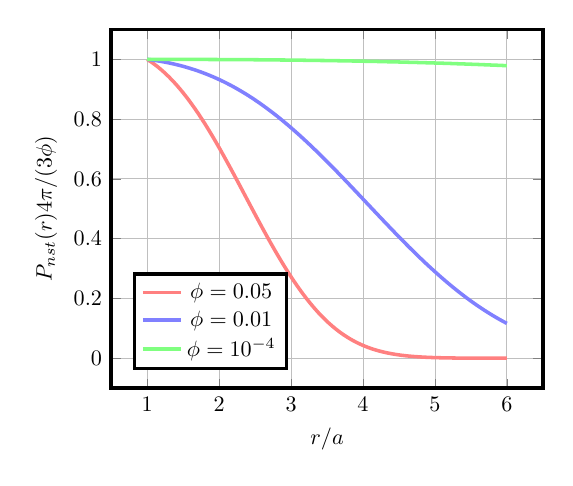
\begin{tikzpicture}[scale=0.8]
    \begin{axis}[
        xlabel={$r/a$},
        ylabel={$P_\text{nst}(r) 4\pi/ (3\phi) $},
        legend style={at={(0.05,0.05)}, anchor=south west},
        grid=major,
        domain=1:6,
        samples=100,
        ultra thick
    ]
    
    % Plot for phi = 0.05
    \addplot[color=red!50,ultra thick]
    { exp(-0.05 * (x^3 - 1))};
    \addlegendentry{$\phi = 0.05$}
    
    % Plot for phi = 0.01
    \addplot[color=blue!50,ultra thick]
    { exp(-0.01 * (x^3 - 1))};
    \addlegendentry{$\phi = 0.01$}
    
    % Plot for phi = 0.001
    \addplot[color=green!50,ultra thick]
    { exp(-0.0001 * (x^3 - 1))};
    \addlegendentry{$\phi = 10^{-4}$}
    
    \end{axis}
\end{tikzpicture}
\hfil
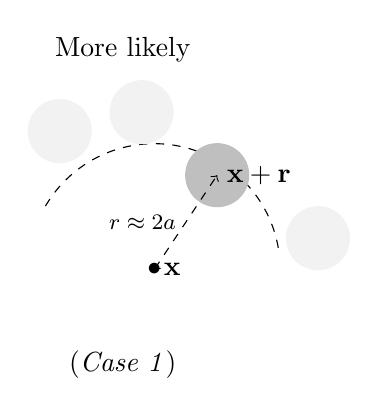
\begin{tikzpicture}[scale=0.8]
  \filldraw[ gray!10!white](+2.6,0.5)circle (0.5);
  \filldraw[ gray!10!white](-1.5,2.2)circle (0.5);
  \draw[dashed](10:2) arc (10:150:2);
  % \filldraw[ gray!50!white](0,0) circle (0.5);
  \filldraw[ gray!50!white](1,1.5)circle (0.5);
  \filldraw[ gray!10!white](-0.2,2.5)circle (0.5);
  \draw(0,0)node{$\bullet$}node[right]{$\textbf{x}$};
  \draw[dashed,<->](0,0)--(1,1.5)node[midway,left]{\footnotesize $r\approx 2 a$}node[right]{$\textbf{x}+\textbf{r}$};
  % \draw[dashed](-0.2,3.5);
  \node[ultra thick] (title) at (-0.5,3.5) {{More likely}};
  \node[ultra thick] (title) at (-0.5,-1.5) {(\textit{Case 1})};
\end{tikzpicture} 
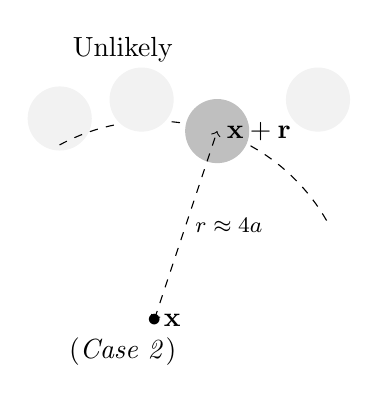
\begin{tikzpicture}[scale=0.8]
  \filldraw[ gray!10!white](+2.6,3.5)circle (0.5);
  \filldraw[ gray!10!white](-1.5,3.2)circle (0.5);
  \draw[dashed](30:3.16) arc (30:120:3.16);
  % \filldraw[ gray!50!white](0,0) circle (0.5);
  \filldraw[ gray!50!white](1,3)circle (0.5);
  \filldraw[ gray!10!white](-0.2,3.5)circle (0.5);
  \draw(0,0)node{$\bullet$}node[right]{$\textbf{x}$};
  \draw[dashed,<->](0,0)--(1,3)node[midway,right]{\footnotesize  $r\approx 4a$}node[right]{$\textbf{x}+\textbf{r}$};
  % \draw[dashed](-0.2,3.5);
  \node[ultra thick] (title) at (-0.5,4.3) {{Unlikely}};
  \node[ultra thick] (title) at (-0.5,-0.5) {(\textit{Case 2})};
\end{tikzpicture} 
\caption{(left) Plot of the normalized nearest neighbor distribution $P_\text{nst}$. 
(right) Sketches explaining the behavior of the nearest neighbor distribution $P_\text{nst}$: 
(\textit{Case 1}) A droplet located at $\textbf{x}+\textbf{r}$ relatively \underline{close} to a point occupied by the continuous phase at \textbf{x}; this situation is likely to happen. 
(\textit{Case 2}) A droplet located at $\textbf{x}+\textbf{r}$ relatively \underline{far} to a point occupied by the continuous phase at \textbf{x}; this situation very unlikely to happen.
Indeed, it implies that no particles are present within the sphere of radius $4a$ centered at $\textbf{x}$ since the nearest neighbor is located at a distance $4a$. 
}
\label{fig:P_nst_f}
\end{figure}
With these assumptions in place, we can compute the \textit{Reynolds stress} using, \ref{eq:relation_ensemble_nst} which reduces to the following formula, 
\begin{equation}
    \avg{\chi_f \textbf{u}_f'\textbf{u}_f'}/\phi_f
    = 
    \frac{3\phi}{4\pi}
    \int_{\mathbb{R}^6}
    \textbf{v}_f^\text{nst}
    \textbf{v}_f^\text{nst}
     e^{-\phi(r^3 -1)}
    d\textbf{r}
    d\textbf{w},
    \label{eq:step_one}
\end{equation}
where it must be understood that $\textbf{v}_f^\text{nst}$ is given by \ref{eq:stokes_sol}. 


Before computing the integration for Stokes flows, we would like to apply this formulation to re-compute the \textit{Reynolds stress} for translating bubbles in potential flows. 
This will allow us to verify the consistency of our methodology. 
Indeed, it can be show that \ref{eq:solution_isolated_at_x} also hols for the \textit{nearest neighbor conditionally averaged} momentum equations in potential flows, thus in that case $\textbf{v}^\text{nst}_f \approx \textbf{u}_f^{1d}$ where we recall that $ \textbf{u}_f^{1d}$ is given by \ref{eq:potential_sol}.
Therefore, we carry out the direct integration of \ref{eq:step_one} using \ref{eq:potential_sol} and obtain, 
\begin{equation}
    \avg{\chi_f \textbf{u}_f'\textbf{u}_f'}
    = \Gamma_\text{inc}(-1,\phi)\phi^2 e^\phi \left\{
        \frac{1}{20}[\textbf{u}_{fp}\textbf{u}_{fp}+ \frac{1}{n_p}\pavg{\textbf{u}_\alpha\textbf{u}_\alpha}]
        + 
        \frac{3}{20} (\textbf{u}_{fp}\cdot \textbf{u}_{fp} + 2k_p)\bm\delta
    \right\},
    \label{eq:potential_nst}
\end{equation}
where $\Gamma_\text{inc}$ is the gamma incomplete function. 
According to \ref{eq:potential_nst} our results differ with \ref{eq:van_wingarden_sol} by a factor of $\Gamma_\text{inc}(-1,\phi)\phi^2 e^\phi$. 
Nevertheless, this inconsistency is easily solved noticing that $\Gamma_\text{inc}(-1,\phi)\phi^2 e^\phi \sim \phi + \mathcal{O}(\phi^2)$. 
Thus, we conclude that at the leading order, our methodology seem consistent with the classical conditional average methodology introduced by \citet{batchelor1972sedimentation}. 

Now that we have all the tools in hand, let us carry out the direct integration of \ref{eq:step_one} for the wake of a spherical droplet in stokes flows. 
Using \ref{eq:solution_isolated_at_x} and \ref{eq:Pnst_explicit} in \ref{eq:step_one} gives, in dimensionless form,  
\begin{equation}
    \avg{\chi_f  \textbf{u}_f'\textbf{u}_f'}^*
    = 
    C_1
    \left\{
        \textbf{u}_{fp}\textbf{u}_{fp}+ \frac{1}{n_p}\pavg{\textbf{u}_\alpha'\textbf{u}_\alpha'}
        -\frac{1}{3} (\textbf{u}_{fp}\cdot \textbf{u}_{fp} + 2k_p)\bm\delta
    \right\},    
    +  C_2
    (\textbf{u}_{fp}\cdot \textbf{u}_{fp} + 2k_p)\bm\delta,
    \label{eq:final_closure}
\end{equation}
with,
\begin{align*}
    C_1(\phi,\lambda)
    = \frac{9(2+3\lambda)^2}{80(1+l)^2}
    % \left[
        \Gamma(1/3) \phi^{2/3}
        % - (27+82\lambda +62\lambda^2)
    % \right]
    ,
    &&
    C_2(\phi,\lambda)
    = \frac{(2+3\lambda)^2}{24(1+l)^2}
    % \left[
        \Gamma(1/3) \phi^{2/3}.
        % - (3+10\lambda +8\lambda^2)
    % \right].
\end{align*}
% \tb{maybe remove order phi terms}
We have decomposed the \textit{Reynolds stress} tensor into two contributions. 
The first term on the right-hand side of \ref{eq:final_closure} is a traceless symmetric tensor, proportional to the functional $C_1$. 
The second term is the isotropic part of the \textit{Reynolds stress} tensor, which is proportional to $C_2$. 

Additionally, we can note that, according to the value of $C_1$ and $C_2$, the \textit{pseudo turbulence} or \textit{Reynolds stress} induced by the translation of the droplets is higher for large values of $\lambda$. 
In other words, a solid particle in translation induces more wake than a bubble of the same size. 

Moreover, as witnessed by the presence of the term $\phi^{2/3}$, in $C_1$ and $C_2$, we conclude that the solution obtained here is still consistent with the observation made in \ref{eq:real_error} or in the previous study \citep{caflisch1985variance}. 
Indeed, for an isolated droplet, i.e. when we take the limit, $\phi \to 0$, we obtain $\lim_{\phi \to 0} \avg{\chi_f \textbf{u}_f' \textbf{u}_f'} / \phi = \infty$. 
Consequently, in agreement with the previous statements, the normalized \textit{Reynolds stress}, i.e. the Reynolds stress divided by the number density or $\phi$,  is infinite for an isolated droplet.
However, when considering a small but finite value of $\phi$ the \textit{Reynolds stress} remains finite and is given by \ref{eq:final_closure}. 

Finally, as it is not the \textit{Reynolds stress} divided by $\phi$ that matter, but $\avg{\chi_f\textbf{u}_f'\textbf{u}_f'}$ itself, note that at the leading order in $\phi$ we obtain,  $\avg{\chi_f\textbf{u}_f'\textbf{u}_f'}\sim\phi^{2/3}$. 
Notably, this trend in $\sim\phi^{2/3}$ is not new and agrees with previous studies found in the literature.
Specifically, in \citet{hill2001first} they compute \textit{Reynolds stress} for ordered array of spheres and found $k_f \sim 0.969 \phi^{2/3}$. 
This nearly agree with our \ref{eq:final_closure} with $\lambda =\infty$ as it gives, $k_f  = 1.50 \phi^{2/3}$.
The difference between our results and \citet{hill2001first}'s result, probably comes from the different particles arrangement considered.  



\subsection{The solution with the consideration of the buoyancy force. }

Although we chose to neglect the source term in \ref{eq:momentum_nst_d_stokes} how can we be certain that it was indeed negligible? 
Even though this term is $\mathcal{O}(\phi)$ in $\textbf{v}^\text{nst}$, it does not necessarily imply that it will contribute at $\mathcal{O}(\phi)$ in $\avg{\rho_f\chi_f \textbf{u}_f'\textbf{u}_f'}$. 
Indeed, in \citet{zhang2021ensemble}, while carrying similar derivations, he found out that the terms of $\mathcal{O}(\phi)$ in the equation for $\textbf{v}^\text{nst}$, contributed to $\mathcal{O}(\phi^{1/3})$ in their final results.  
Thus, in this section we carry out the same calculation, but with the consideration of the buoyancy source term. 

\subsubsection{The velocity fields singularity solution}

Since the velocity field $\textbf{v}^\text{nst}$ still satisfy the linear Stokes equations, we may proceed into two steps. 

First, regardless of the right-hand side of \ref{eq:momentum_nst_d_stokes} the boundary condition at the surface of the particle, located at \textbf{y}, will generate the velocity fields \citep{pozrikidis1992boundary}, 
\begin{equation}
    \textbf{v}^\text{nst}_1[\textbf{z},t|\textbf{x},\textbf{w},\textbf{y}]
    = 
    \frac{a}{4}(\textbf{w}- \textbf{u}[\textbf{y},t])\cdot\left[
        \frac{2+3\lambda}{1+\lambda}
        +
        a^2\frac{\lambda}{2(1+\lambda)}\pddz^2 
    \right]\mathcal{G}(\textbf{z},\textbf{y}).
    \label{eq:solution_isolated2}
\end{equation}

Secondly, let us turn our attention to the source term on the right-hand side of \ref{eq:momentum_nst_d_stokes}. 
Following \citet{zhang2021ensemble}, we remark that the contribution to the velocity field, generated by the particle-free zone, can be written as a sum of \textit{Stokeslets} of magnitude $\phi\Delta \rho \textbf{g}$.
Indeed, since the Dirac delta function is a unit of convolution product, we may write, 
\begin{equation}
    \phi \Delta\rho  \textbf{g} H(|\textbf{y} - \textbf{x}| - |\textbf{z} - \textbf{x}|)
    = 
    \phi \Delta\rho  \textbf{g} 
    \int_{|\textbf{y} - \textbf{x}| > |\textbf{x}' - \textbf{x}|}
    \delta(\textbf{x}'-\textbf{z})
    d\textbf{x}'. 
\end{equation}
Additionally, the velocity field evaluated at \textbf{z}, generated by the point force,  $\phi\Delta \rho \textbf{g}\delta(\textbf{x}' - \textbf{z})$, can be written \citep{pozrikidis1992boundary}, 
\begin{equation}
    \frac{\phi\Delta \rho \textbf{g}}{8\pi \mu_f}\cdot \mathcal{G}(\textbf{z} - \textbf{x}')
\end{equation}
where $\mathcal{G}(\textbf{r})$ is the Green function of the Stokes equations, namely, 
\begin{equation}
    \mathcal{G}(\textbf{r}) = \frac{\bm\delta}{r} + \frac{\textbf{rr}}{r^3}.
\end{equation}
Consequently, the velocity fields generated by the right-hand-side of \ref{eq:momentum_nst_d_stokes}, meaning by particle-free zone, as given in \ref{fig:unst}, can be written as, 
\begin{equation}
    \textbf{v}_b^\text{nst}[\textbf{z},t|\textbf{y},\textbf{w},\textbf{x}]
    = 
    \frac{\phi\Delta \rho \textbf{g}}{8\pi \mu_f}\cdot 
    \int_{|\textbf{x}'-\textbf{x}|< |\textbf{y}- \textbf{x}|}
    \mathcal{G}(\textbf{z},\textbf{x}')
    d\textbf{x}'
    \label{eq:v_b_sol}
\end{equation}
where we used the subscript $_b$ to denote the particle-free zone contribution. 
Due to the linearity of the Stokes equations, the total velocity field is thus the sum of \ref{eq:solution_isolated2} and \ref{eq:v_b_sol}. 
% Likewise, the stress generated by the particle-free-zone might be written \citep{pozrikidis1992boundary},
% \begin{equation}
%     \bm\sigma_b^\text{nst}[\textbf{z},t|\textbf{y},\textbf{w},\textbf{x}]
%     = 
%     \frac{\phi\Delta \rho \textbf{g}}{8\pi}\cdot 
%     \int_{|\textbf{x}'-\textbf{x}|< |\textbf{y}- \textbf{x}|}
%     \mathcal{T}(\textbf{z},\textbf{x}')
%     d\textbf{x}'
%     \label{eq:sigma_b_sol}
% \end{equation}
% with, 
% \begin{equation}
%     \mathcal{T}(\textbf{z},\textbf{x}')
%     = - 6\frac{\textbf{rrr}}{r^5}. 
% \end{equation}
% Here, $\textbf{r} = \textbf{z} - \textbf{x}'$. 

Therefore, the total velocity field $\textbf{v}^\text{nst}_f$ at the point $\textbf{x}$, can be obtained using \ref{eq:v_b_sol} and \ref{eq:solution_isolated2} evaluated at the point \textbf{x}, and  \ref{eq:reformulation}, which yields,  
\begin{multline}
    \textbf{v}^\text{nst}_f [\textbf{x},\textbf{w},\textbf{y},t]
    =
    \frac{a}{4}(\textbf{w}- \textbf{u}[\textbf{y},t])\cdot\left[
        \frac{2+3\lambda}{1+\lambda}
        +
        a^2\frac{\lambda}{2(1+\lambda)}\grad^2 
    \right]\mathcal{G}(\textbf{x},\textbf{y})\\
    +
    \phi(\textbf{u}_d - \textbf{u}_f)
    + 
    \frac{\phi\Delta \rho \textbf{g}}{8\pi \mu_f}\cdot 
    \int_{|\textbf{x}'-\textbf{x}|< |\textbf{y}- \textbf{x}|}
    \mathcal{G}(\textbf{x},\textbf{x}')
    d\textbf{x}',
\end{multline}
Carrying out the integral on the second line gives directly,
\begin{equation}
    \int_{|\textbf{x}'-\textbf{x}|< |\textbf{y}- \textbf{x}|}
    \mathcal{G}(\textbf{x},\textbf{x}')
    d\textbf{x}'
    = \frac{8\pi}{3}|\textbf{x}- \textbf{y}|^2\bm\delta
\end{equation}
which finally gives the result, 
\begin{multline}
    \textbf{v}^\text{nst}_f
    =
    \frac{a}{4}(\textbf{w}- \textbf{u}_f[\textbf{y},t])\cdot\left[
        \frac{2+3\lambda}{1+\lambda}
        +
        a^2\frac{\lambda}{2(1+\lambda)}\grad^2 
    \right]\mathcal{G}(\textbf{x},\textbf{y})
    + 
    \frac{\phi\Delta \rho \textbf{g}}{3\mu_f} |\textbf{x}-\textbf{y}|^2
    +
    \mathcal{O}(\phi).
    \label{eq:final_sol_v_nst}
\end{multline}
Note that we neglected the $\mathcal{O}(\phi)$ terms however we must keep the buoyancy term as it is of $\mathcal{O}(|\textbf{x}-\textbf{y}|^2\phi)$ which remains significant far from the droplet. 
In this expression, we clearly identify $2$ distinct contributions. 
The first two terms on the right-hand side of \ref{eq:final_sol_v_nst} correspond to the disturbance field generated by an isolated droplet, which was the only contribution in \ref{eq:solution_isolated_at_x}. 
The third term corresponds to the ``backflow velocity'' as called by \citet{zhang2021ensemble}, it refers to the flow generated by the particle-free zone, due to buoyancy forces. 
% Finally, the last term ensure that we stay in the right reference frame. 
Note that in \citet[Appendix A]{zhang2021ensemble} they carried out nearly the same calculation for solid particles.
One can note a small differences between \ref{eq:final_sol_v_nst} with $\lambda = \infty$ and Eq. (B 4) of  \citet[Appendix A]{zhang2021ensemble} , indeed, while we have got$(\textbf{w}- \textbf{u}_f[\textbf{y},t])$ as factor of the first term, he obtained $(\textbf{w}- \textbf{u}_f - \textbf{v}_b^\text{nst})$. 
This is due to the different reference frames used for the velocity fields.
Indeed, here we solved for $\textbf{v}^\text{nst}$ while in \citet{zhang2021ensemble} they solve for $\textbf{u}^\text{nst}$. 
The consequence is that, while we have only one source term at the right-hand side of \ref{eq:momentum_nst_d_stokes}, \citet{zhang2021ensemble} has a supplementary, constant source term overall the domain. 
This is the reason for the presence of his $\textbf{v}_b'$ which is not present in \ref{eq:final_sol_v_nst}. 
Thus, our result is consistent with \citet{zhang2021ensemble}, moreover, we generalized and demonstrated his results for spherical droplets. 


For a better physical understanding, we present now the dimensionless form of \ref{eq:final_sol_v_nst}. 
The lengths are made dimensionless using the radius of the particle $a$, the velocity vector $\textbf{w} - \textbf{u}_f$ is made dimensionless the norm $U = |\textbf{w} - \textbf{u}_f|$, 
Thus, we introduced the unit vector: $\textbf{e} = \textbf{w} - \textbf{u}_f/U$. 
Likewise, the gravity acceleration vector is made dimensionless using its norm, such that the unit vector in the direction of the acceleration of gravity is given by $\textbf{k} = \textbf{g} / g$, with $g = |\textbf{g}|$. 
Dividing \ref{eq:final_sol_v_nst} by $U$ and using these definitions yields directly the dimensionless expression for the disturbance velocity field, 
\begin{equation}
    \frac{\textbf{v}^\text{nst}_f}{U}
    =
    \frac{1}{4}\textbf{e}\cdot\left[
        \frac{2+3\lambda}{1+\lambda}
        +
        \frac{\lambda}{2(1+\lambda)}\grad^2 
    \right]\mathcal{G}(\textbf{x},\textbf{y})
    + \phi A |\textbf{x}-\textbf{y}|^2 \textbf{k}
    + \mathcal{O}(\phi). 
    \label{eq:v_nst_solution_adim}
\end{equation}
Note that where we kept the same notations for all the distances vector, however, they are assumed dimensionless in this expression. 
Additionally, we introduced the dimensionless number, 
\begin{equation}
    A = \frac{Ga^2}{12 Re}=\frac{\Delta \rho g (2a)^2}{12 \mu_f U}
    \label{eq:A_general}
\end{equation}
where we recall that $Ga$ is the \textit{Galileo} number and $Re$ the \textit{Reynolds} number, defined as,  
\begin{align*}
    Re= \frac{\rho_f U 2a}{\mu_f},
    &&
    Ga^2 = \frac{\rho_f \Delta\rho g (2a)^3}{\mu_f^2},
\end{align*}
respectively. 
Upon considering specific scenarios, such as a steady state buoyant rising droplet, one is able to relate $Ga$ and $Re$ and give an explicit expression for the term $A$.
 



\subsubsection{The pseudo turbulent tensor closure}

From \ref{eq:v_nst_solution_adim} we may already compute the integral in \ref{eq:step_one}. 
However, as $\textbf{e}$ and $\textbf{k}$ in \ref{eq:v_nst_solution_adim}  are not necessarily collinear vectors, the functional form of the resulting stress tensor is not trivial. 
Indeed, since $\textbf{v}_f^\text{nst}\sim \textbf{e}$ and $\sim \textbf{k}$, the final results must be a tensor built from sums of products of these two vectors.  
Additionally, since $\avg{\rho_f \textbf{u}_f'\textbf{u}_f'}$ is a symmetric tensor, the result must be a symmetric tensor as well. 
The only second-order symmetric tensors that can be constructed from the  two arbitrary vectors: $\textbf{e}$ and $\textbf{k}$ are, 
\begin{align*}
    \textbf{ee}
    && (\textbf{e}\cdot \textbf{e})\bm\delta, 
    && \textbf{kk},
    && (\textbf{k}\cdot \textbf{k})\bm\delta,
    && \textbf{ke}+\textbf{ek},
    && (\textbf{k}\cdot \textbf{e})\bm\delta, 
\end{align*}
we deduce that the volume integral of \ref{eq:step_one}, have the form, 
\begin{align}
    \frac{1}{U^2}
    \frac{3\phi}{4\pi}\int_{\mathbb{R}^3}
    \textbf{v}_f^\text{nst}
    \textbf{v}_f^\text{nst}
     e^{-\phi(r^3 -1)}
    d\textbf{r}
    &= C^{(1)}_e \left[
        \textbf{ee}
         - \frac{1}{3}(\textbf{e}\cdot \textbf{e})\bm\delta
    \right]
    + C^{(2)}_e 
    (\textbf{e}\cdot \textbf{e})\bm\delta \nonumber \\
    &+ C^{(1)}_k \left[
        \textbf{kk}
         - \frac{1}{3}(\textbf{k}\cdot \textbf{k})\bm\delta
    \right]
    + C^{(2)}_k 
    (\textbf{k}\cdot \textbf{k})\bm\delta \nonumber \\
    &+ C^{(1)}_{ek} \frac{1}{2}\left[
        (\textbf{ek}  + \textbf{ke})
         - \frac{2}{3}(\textbf{k}\cdot \textbf{e})\bm\delta
    \right]
    + C^{(2)}_{ek} 
    (\textbf{e}\cdot \textbf{k})\bm\delta 
    \label{eq:functional_form}
\end{align}
where the first term of each line correspond to symmetric traceless tensors, and the second term of each line to the corresponding isotropic contribution. 
The first two constant, $C^{(1)}_e$ and $C^{(2)}_e$ can be obtained setting $\textbf{k}= 0$ in \ref{eq:v_nst_solution_adim} and performing the integration. 
Likewise, $C^{(1)}_k$ and $C^{(2)}_k$ can be obtained setting $\textbf{e}=0$ in \ref{eq:v_nst_solution_adim}. 
The constants, $C^{(1)}_{ek}$ and $C^{(2)}_{ek}$ can be obtained setting $\textbf{g} = 0$ in of the $\textbf{v}_f^\text{nst}$ on the left-hand side of \ref{eq:functional_form} and $\textbf{e}=0$ in the other $\textbf{v}_f^\text{nst}$. 
Thus, we obtain at the leading order, 
\begin{align}
    C_e^{(1)} =
    % \frac{9(2+3\lambda)^2 \Gamma(\frac{1}{3})}{80(\lambda+1)^2}\phi^{2/3}
    \frac{27}{10}
    C_e^{(2)}
    % + \mathcal{O}(\phi)
    &&  C_e^{(2)} =
    \frac{(2+3\lambda)^2 \Gamma(\frac{1}{3})}{24(\lambda+1)^2}\phi^{2/3}
    + \mathcal{O}(\phi)
    \\
    C_k^{(1)} =
    % A^2 \Gamma\left(7/3\right)\phi^{2/3}
    3
    C_k^{(2)}
    % + \mathcal{O}(\phi^{5/3})
    && C_k^{(2)} =
    A^2 \frac{\Gamma(\frac{7}{3})}{3}\phi^{2/3}
    + \mathcal{O}(\phi^{5/3})
    \\
    C_{ek}^{(1)} =
    3
    C_{ek}^{(2)}
    % A\frac{2 (2+3\lambda) \Gamma(\frac{4}{3})}{3 (\lambda+1)}\phi^{2/3}
    % + \mathcal{O}(\phi^{4/3})
    && C_{ek}^{(2)} =
    A\frac{2 (2+3\lambda) \Gamma(\frac{4}{3})}{9(\lambda+1)}\phi^{2/3}
    + \mathcal{O}(\phi^{4/3})
    \label{eq:constants}
\end{align}
Note that $C_e^{(1)}$ and $C_e^{(2)}$ correspond to the constants obtained in \ref{eq:final_closure}. 
Additionally, note that the leading order contribution from the backflow velocity is $\sim \phi^{2/3}$ as well. 
Therefore, these new terms are non-negligible in this general framework. 


Following \ref{eq:step_one}, to obtain the ensemble-averaged \textit{Reynolds stress} tensor we now integrate  \ref{eq:functional_form} over all the $\textbf{w}$.
This yields the final form of our \textit{Pseudo turbulent} tensor model, namely, 
\begin{align}
    \frac{\avg{\chi_f \textbf{u}_f'\textbf{u}_f'}}{\phi_f U^2}
    &= 
    C^{(1)}_e \left[
        \textbf{e}_p\textbf{e}_p
        + \frac{\pavg{\textbf{u}_\alpha'\textbf{u}_\alpha'}}{n_p U^2}
         - \frac{1}{3}(\textbf{e}_p\cdot \textbf{e}_p+2k_p/U^2)\bm\delta
    \right]
    + C^{(2)}_e 
    (\textbf{e}_p\cdot \textbf{e}_p+2k_p/U^2)\bm\delta \nonumber \\
    &+ C^{(1)}_k  \left[
        \textbf{kk}
         - \frac{1}{3}(\textbf{k}\cdot \textbf{k})\bm\delta
    \right]
    +C^{(2)}_k 
    (\textbf{k}\cdot \textbf{k})\bm\delta \nonumber \\
    &+ C^{(1)}_{ek} \left[
        \frac{1}{2}
        (\textbf{e}_p\textbf{k}  + \textbf{k} \textbf{e}_p)
         - \frac{1}{3}(\textbf{k}\cdot \textbf{e}_p)\bm\delta
    \right]
    + C^{(2)}_{ek}
    (\textbf{e}_p\cdot \textbf{k})\bm\delta 
    \label{eq:functional_form_avg}
\end{align}
In this expression $\textbf{e}_p = \int \textbf{e} d\textbf{w} $ represents the mean direction of the mean relative phase velocity $\textbf{u}_{pf}$ such that $\textbf{u}_{pf} = U \textbf{e}_p$, in opposition to $\textbf{e}$ which represented the direction of a single particle relative velocity. 



In summary, the only additional terms appearing due to the integration over the velocity phase space is the addition of the particle fluctuation contribution to the \textit{Reynolds stress}. 
However, it is likely that $k_p/U^2 \sim \phi$ at least, therefore at $\mathcal{O}(\phi)$ and at low $\mathcal{O}(Re)$ this term might be safely neglected. 
This statement will be confirmed later on. 



\subsubsection{Steady-state rising droplet}

Let us now study the case where $\textbf{k} = - \textbf{e} = \textbf{e}_z$, meaning that the droplet rises in the opposite direction of gravity which is acting in the vertical direction denoted by $\textbf{e}_z$.  
At $\mathcal{O}(\phi)$ and in Stokes flow regime, the drag applied on a spherical droplet is given by the formula of Hadamard-Ribczynski.
Thus, the magnitude of the steady-state rising velocity of a droplet is given by, 
\begin{equation}
    U = \Delta \rho \frac{g (2a)^2}{6 \mu_f }\left(\frac{1+\lambda}{2+3\lambda}\right).
    \label{eq:U_isolated}
\end{equation}
% \begin{equation}
%     2a \pi \mu_f \left(\frac{3\lambda +2}{\lambda +1}\right) 
%     U
%     = 
%     \frac{4}{3}\pi a^3 
%     \Delta \rho
%     g,
% \end{equation}
We deduce from this relation that in this specific situation, i.e. when the direction of the relative velocity \textbf{e} is aligned with the gravity acceleration direction, we have, 
\begin{equation}
    A = \frac{1}{2}\left(\frac{3\lambda +2}{\lambda +1}\right). 
    \label{eq:closure_A}
\end{equation}
Injecting this expression into \ref{eq:v_nst_solution_adim} gives us an explicit expression of the velocity field $\textbf{v}^\text{nst}_f$. 

To give a better idea of the meaning of $\textbf{v}_f^\text{nst}$, we display 
in \ref{fig:vnst_vertical} the streamlines generated by the field $\textbf{v}_f^\text{nst}(\textbf{r})$ in the cross-section, given by the plane formed by the vectors $(\textbf{e}_x,\textbf{e}_z)$. 
\begin{figure}[h!]
    \centering
    \includegraphics[height = 0.33\textwidth]{image/Vnst_l_10_0.pdf}
    \includegraphics[height = 0.33\textwidth]{image/Vnst_l_10_1.pdf}
    \includegraphics[height = 0.33\textwidth]{image/Vnst_l_10_5.pdf}
    % \includegraphics[height = 0.33\textwidth]{image/Vnst_l_10_10.pdf}
    \caption{Streamlines of the disturbance velocity field $\textbf{v}_f^\text{nst}(\textbf{r}_f)$ \eqref{eq:v_nst_solution_adim}  in the cross-section given by the plane $(\textbf{e}_x,\textbf{e}_z)$, for multiples volume fraction $\phi = 0, 0.01$ and $0.05$ at $\lambda = 10$.  
    The color map indicates the magnitude of the velocity, from black which corresponds to a velocity magnitude of 0, to the color at the interface which corresponds to 1.
    In this situation $\textbf{e} = \textbf{e}_z$ and $\textbf{k} = -\textbf{e}_z$}
    \label{fig:vnst_vertical}
\end{figure}
We can observe on \ref{fig:vnst_vertical} (left) that $\textbf{v}^\text{nst}_f(\phi =0)$ corresponds to the disturbance field of an isolated particle in Stokes flow. 
This is easily understandable considering that the last term on the right-hand side of \ref{eq:v_nst_solution_adim} cancel for $\phi=0$, thus leaving us with an expression equivalent to \ref{eq:solution_isolated}, which is the disturbance field of an isolated particle. 
At finite volume fraction, $\phi =0.01$, we  observe in \ref{fig:vnst_vertical} (middle), that a downstream velocity starts to appear at a large distance from the particle center.  
As discussed previously, this ``backflow velocity'' is given by the term $\phi A |\textbf{x}- \textbf{y}|^2 \textbf{k}$ in \ref{eq:solution_isolated}.
The particle is thus surrounded by a spherical shell within which the disturbance field has a positive vertical velocity, and outside which the velocity is negative.
In the following discussion, we call this spherical shell the \textit{confinement zone}.   
For higher volume fractions ($\phi = 0.05$), the backflow velocity is even stronger leading to a smaller confinement zone around the particle. 

Let us discuss the form of \ref{eq:functional_form_avg} in the specific case displayed in \ref{fig:vnst_vertical}, i.e. spherical droplets rising in stokes flow. 
Since $\textbf{e}_p = - \textbf{k}$ we have $\textbf{e}_p\textbf{k} = - \textbf{kk}$. 
Additionally, one can use \ref{eq:closure_A} into the expression for $C_k^{(1)}$ and $C_{ek}^{(1)}$. 
In this specific case, by carrying out the calculation, we obtain, 
\begin{equation}
    C_k^{(1)} \textbf{kk} + C_{ek}^{(1)} \textbf{ke}_p
    = 0. 
    \label{eq:cancelation1}
\end{equation}
Applying the same reasoning, one can also deduce that, 
\begin{equation}
    C_k^{(2)} \textbf{k}\cdot \textbf{k} + C_{ek}^{(2)} \textbf{k}\cdot \textbf{e}_p
    = 0. 
    \label{eq:cancelation2}
\end{equation}
Consequently, we must deduce that the contribution from the gravity acceleration to the \textit{Reynolds stress} tensor, remains zero in this simplified situation. 
This might seem surprising considering the seemingly non-negligible action of the gravity on the velocity field displayed \ref{fig:vnst_vertical}. 
However, we must understand from this, that the velocity variance generated by the backflow velocity, also induces a decrease of the velocity variance generated by the particle motion compared to the isolated case.
In other words, the backflow velocity generated at the boundaries of the confinement zone a low-velocity variance, which is exactly balanced by the velocity variance generated by the backflow at the exterior of the confinement zone.    
Note that this explanation is only true when $\textbf{k} = - \textbf{e}_p$. 

In the next section we examine a situation where the velocity of the dispersed phase is not in the opposite direction of gravity. 



\subsubsection{Horizontal motions}

We now consider the case were $\textbf{e}_p = \textbf{e}_x$, and $\textbf{k} = - \textbf{e}_z$, where $\textbf{e}_z$ is still the vertical unit vector and $\textbf{e}_x$ the Horizontal unit vector. 
Of course, in the steady-state regime and isolated from the boundary of the domain, $\textbf{e}_p$, cannot be otherwise than vertical. 
However, in a more general case, $\textbf{e}_p$ have absolutely no reason to be in the vertical direction, due to boundaries or transient effects. 
In this case, $A$ is given by \ref{eq:A_general} and requires the norm of the relative velocity $U$ to be computed.

\begin{figure}[h!]
    \centering
    \includegraphics[height = 0.33\textwidth]{image/Vnst_H_l_10_0.pdf}
    \includegraphics[height = 0.33\textwidth]{image/Vnst_H_l_10_1.pdf}
    \includegraphics[height = 0.33\textwidth]{image/Vnst_H_l_10_5.pdf}
    % \includegraphics[height = 0.33\textwidth]{image/Vnst_l_10_10.pdf}
    \caption{Streamlines of the disturbance velocity field $\textbf{v}^\text{nst}(\textbf{r}_f)$  \eqref{eq:v_nst_solution_adim} in the cross-section given by the plane $(\textbf{e}_x,\textbf{e}_z)$, for multiples volume fraction $\phi = 0, 0.01$ and $0.05$ at $\lambda = 10$.  
    The color map indicates the magnitude of the velocity, from black which corresponds to a velocity magnitude of 0, to the color at the interface which corresponds to 1.
    In this situation $\textbf{e} = \textbf{e}_x$ and $\textbf{k} = -\textbf{e}_z$.
    The constant $A$ have been arbitrarily set to $1$. }
    \label{fig:vnst_horizontal}
\end{figure}
In \ref{fig:vnst_horizontal} we display the streamlines generated by the velocity field $\textbf{v}_f^\text{nst}$. 
As before, we remark that at $\phi = 0$, $\textbf{v}_f^\text{nst}$ corresponds to the disturbance velocity field of an isolated droplet translating horizontally in Stokes flow. 
At $\phi = 0.01$, see \ref{fig:vnst_horizontal} (middle), the effect of gravity induces a downstream backflow, this time, it is not in the opposite direction of the disturbance velocity of the drop.
At higher volume fractions this downstream flow is stronger, and the confinement zone around the particle is smaller. 
In short, we observe the same phenomenon as in the situation reported on \ref{fig:vnst_vertical}, except that the droplet disturbance field is not in the opposite direction of the backflow velocity. 

In this situation, the relation given by \ref{eq:cancelation1} and \ref{eq:cancelation2} are not true anymore. 
Thus, in this case, the \textit{Reynolds stress} tensor is given by, 
\begin{equation}
    \frac{\avg{\chi_f \textbf{u}_f'\textbf{u}_f'}}{\phi_f U^2}
    = 
    C^{(1)}_e 
    \textbf{e}_x\textbf{e}_x
    % + \frac{\pavg{\textbf{u}_\alpha'\textbf{u}_\alpha'}}{n_p U^2}
    +C^{(1)}_k    
    \textbf{e}_z\textbf{e}_z
    - C^{(1)}_{ek} 
        \frac{1}{2}
        (\textbf{e}_x\textbf{e}_z+ \textbf{e}_z \textbf{e}_x)
    + [C^{(2)}_e + C^{(2)}_k - (C^{(1)}_k + C^{(1)}_e )/3 ]  \bm\delta. 
\end{equation}
The contribution from the wake of the particles is still present and is given by $C_e^{(1)}$ and $C_e^{(2)}$. 
This contribution is aligned with the direction of the droplet velocity, $\textbf{e}_x\textbf{e}_x$. 
Regarding the buoyancy forces, it provides an additional contribution that is proportional to $\textbf{e}_z\textbf{e}_z$. 
Finally, the cross terms $\textbf{e}_p \textbf{k}$ provide off-diagonal terms proportional to $\textbf{e}_z \textbf{e}_x$ or $\textbf{e}_x \textbf{e}_z$. 
The isotropic part of this tensor is the sum of the aforementioned contributions. 
Consequently, this proves that the Reynolds stress tensor posses off diagonal terms given by $C^{(1)}_{ek} 
\frac{1}{2} (\textbf{e}_x\textbf{e}_z+ \textbf{e}_z \textbf{e}_x)$ , that are related to the correlation of the backflow with the droplet disturbance field. 

\subsection{Discussion}

In this section, we have considered the translating motion of a spherical droplet in Stokes flow. 
The \textit{Reynolds stress} closure obtained is a function of $\textbf{u}_{fp}$ the relative phase velocity and the direction of the buoyancy force $\textbf{g}$. 
In the low inertia and dilute regime, we have shown that the ambient body force field $\textbf{g}$ plays a non-negligible role on the \textit{Nearest Neighbor Conditional Averaged} disturbance fields.
When the droplet translation is vertical (in the opposite direction of gravity) the terms related to the buoyancy force turn out to cancel out in the \textit{Reynolds stress} closure.
However, we have shown that it is not the case when the droplet's mean motion were not aligned with the direction of gravity.  

To extend this model, one must consider a more general ambient field, not only a uniform velocity field as demonstrated in this section, but mean shearing motions, or quadratic flows and so on. 
This will be the purpose of the last section of this chapter. 
Nevertheless, as this theoretical approach is new, we focus on numerically validating this model as a first step. 
